\section{INTRODUÇÂO}

Segundo \cite{pegado_flutter_2006}, o \emph{flutter} de painéis é um
fenômeno de grande desafio e interesse no voo supersônico e 
hipersônico. Em trabalho desenvolvido anteriormente por 
\cite{santos_finite_2019}
obteve-se uma ferramenta de 
pré-processamento, geração de malha aerodinâmica e pós-processamento
para a análise aeroelástica de \emph{flutter} para o NASTRAN, um 
conjunto de códigos destinado à análise em elementos finitos 
amplamente utilizado no setor aeroespacial.

Neste artigo é primeiramente realizado um estudo das capacidades do 
MSC/NASTRAN para a modelagem 
aeroelástica e análise de \emph{flutter}.

A escolha do MSC/NASTRAN para o estudo vem de seu longo 
desenvolvimento no setor aeroespacial desde a abertura do código 
original pela NASA \citep[p. 1]{macneal_organizational_1974}, que 
hoje contém funcionalidades modernas além de
manter funcionalidades coexistentes a outros derivados do NASTRAN 
mantendo-se a reprodutibilidade do conteúdo.
Neste estudo verifica-se quais os modelos aerodinâmicos, de 
interpolação e solução do problema de autovalor de \emph{flutter} 
presente no MSC/NASTRAN.

Posteriormente, é descrito a metodologia para um estudo de 
convergência de malha e para a análise de
um caso de placa em material composto laminado, utilizando-se da Teoria Pistão.

Os resultados obtidos são discutidos e 
comparados com referências da literatura nas seções seguintes.


\section{ESTUDO DAS CAPACIDADES DO NASTRAN}

A análise de estabilidade aeroelástica no MSC/NASTRAN, utilizando-se a solução 145, possui três áreas que são requeridas a atenção do usuário: a modelagem aerodinâmica; a interpolação entre as malhas estruturais e aerodinâmicas; e o método de solução aeroelástica. Nas próximas subseções cada área é discutida com um foco no problema apresentado.

\subsection{Modelagem Aerodinâmica}

O MSC/NASTRAN possui sete métodos de obtenção das matrizes aerodinâmicas: o 
\emph{Doublet-Lattice Method} (DLM); o \emph{ZONA51} ou \emph{Harmonic Gradient Method} (HGM); o \emph{Constant Pressure Method} (CPM); o DLM com
interferência asa-fuselagem; o \emph{Mach Box Method} (MBM); o \emph{Strip Theory};
e o \emph{Piston Theory} (ou Teoria Pistão).
Todos os métodos suportam um escoamento não estacionário, se diferenciando
em relação à teoria aerodinâmica aplicada, validade de condições do escoamento,
método de discretização, dentre outros detalhes pertinentes a cada método
\citep[p. 17]{patrannastran_aeroelastic_2019}.

Um resumo das principais características de cada método está disposto na Tabela 
\ref{nastran-table}, excluindo-se o DLM com interferência asa-fuselagem, já que sua aplicação foge
ao escopo deste trabalho. 

\begin{table}[H]
\centering
\caption{Resumo de características dos métodos aerodinâmicos.}
\begin{tabular}{|c|c|c|c|}
\hline
\textbf{Método} & \textbf{Teoria Aerodinâmica}                                                          & \textbf{Discretização} & \textbf{Validade de Mach} \\ \hline
DLM             & Potencial Linearizada                                                                 & \emph{Boxes}                  & Subsônico                 \\ \hline
HGM    & \begin{tabular}[c]{@{}c@{}}Supersônico\\ Potencial Linearizada\end{tabular}           & \emph{Boxes}                  & $\num{1.2} < M < \num{3.0}$           \\ \hline
CPM             & \begin{tabular}[c]{@{}c@{}}Supersônico\\ Potencial Linearizada\end{tabular}           & \emph{Boxes}                  & $\num{1,1} < M < \num{3,0}$           \\ \hline
MBM             & \begin{tabular}[c]{@{}c@{}}Supersônico\\ Potencial Linearizada\end{tabular}           & \emph{Boxes}                  & $\num{1.2} < M < \num{3.0}$           \\ \hline
\emph{Strip Theory}    & Potencial Linearizada                                                                 & \emph{Strips}                 & Subsônico                 \\ \hline
\emph{Piston Theory}   & \begin{tabular}[c]{@{}c@{}}Pistão de 3ª Ordem\\ com correção de Van Dyke\end{tabular} & \emph{Strips}                 & $\num{2,5} < M < \num{7,0}$           \\ \hline
\end{tabular}
\fonte{\cite{liu_recent_1996} e \cite{patrannastran_aeroelastic_2019}}
\label{nastran-table}
\end{table}

Algumas características são importantes para se entender a Tabela \ref{nastran-table}.
As teorias aerodinâmicas potenciais linearizadas não levam em consideração a espessura do perfil aerodinâmico, o que não é desejável, já que a espessura tem um efeito de reduzir a velocidade de \emph{flutter}. Tal fato não ocorre no método \emph{Piston Theory} que possibilita a correção para espessura.

A discretização em \emph{Boxes} é disposta como um \emph{grid} planar de elementos retangulares
ou triangulares como indicado na Figura \ref{fig-boxes}.
Duas diferenças são notáveis: no método CPM não é possível utilizar elementos triangulares;
e no método MBM o usuário deve definir os geometria da superfície aerodinâmica e a rotina computará os elementos que, por sua vez, possuirão sua 
diagonal paralela a linha de Mach, tal como ilustrado na Figura \ref{fig-mach-boxes}.
Nestas formulações há a influência aerodinâmica entre os elementos.

\begin{figure}[H]
\centering
\caption{Discretização em \emph{Boxes}.}
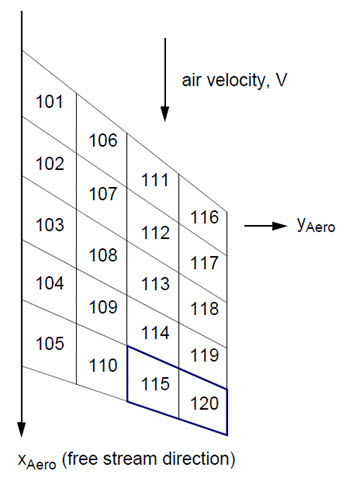
\includegraphics[width=0.4\linewidth]{figures/boxes.png}
\fonte{\cite{patrannastran_aeroelastic_2019}}
\label{fig-boxes}
\end{figure}

\begin{figure}[H]
\centering
\caption{Discretização em \emph{Boxes} para o método MBM.}
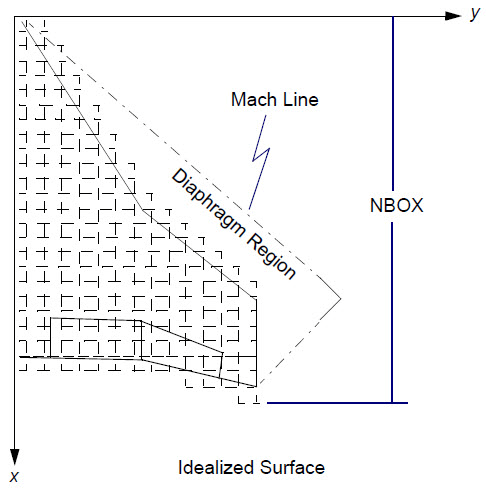
\includegraphics[width=0.5\linewidth]{figures/mach-boxes.png}
\fonte{\cite{patrannastran_aeroelastic_2019}}
\label{fig-mach-boxes}
\end{figure}

Já a discretização em \emph{Strips} (ou faixas)  é a disposição de faixas coplanares como ilustrado na Figura \ref{fig-strips}, nestas formulações não há influência aerodinâmica entre as faixas.

\begin{figure}[H]
\centering
\caption{Discretização em \emph{Strips}.}
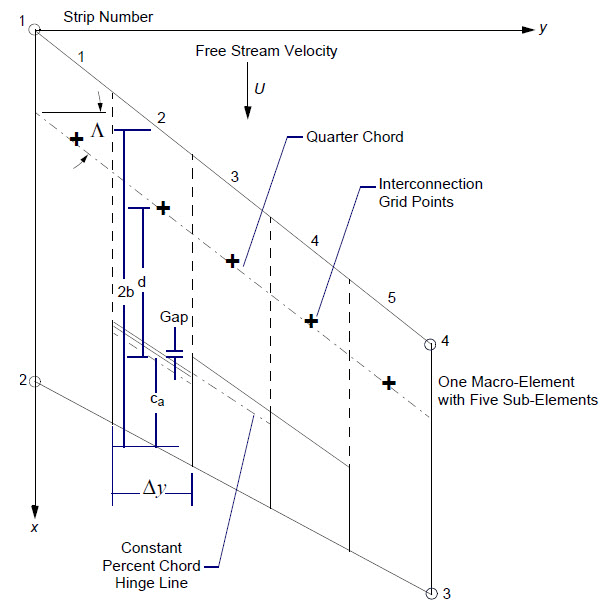
\includegraphics[width=0.5\linewidth]{figures/strip.png}
\fonte{\cite{patrannastran_aeroelastic_2019}}
\label{fig-strips}
\end{figure}

Além disto, alguns métodos possibilitam a modelagem de superfícies de controle, correções para enflechamento (\emph{sweep angle}), compressibilidade, dentre outras propriedades. Tais possibilidades não serão discutidas por fugirem do escopo deste trabalho.

Os métodos apresentam restrições quanto à sua utilização. Na Tabela \ref{nastran-table} verificamos em qual regime de número de Mach cada método se enquadra. Há também restrições de natureza geométrica: no \emph{Piston Theory} é preciso que a corda se mantenha rígida, isto é, sem deformações.

\subsection{Interpolação Aerodinâmica-Estrutural}

Para se obter as matrizes aerodinâmicas e estruturais acopladas, é necessário a interpolação entre os deslocamentos e forças nodais entre as malhas aerodinâmica e estrutural. Para tanto o MSC/NASTRAN fornece cinco métodos de interpolação, totalizando dez opções de solução, contudo, são dois os mais relevantes para o problema aqui apresentado: o \emph{Surface Spline}; e o \emph{Linear Spline}.

\begin{figure}[H]
\centering
\caption{Métodos de interpolação \emph{Surface Spline} e \emph{Linear Spline}.}
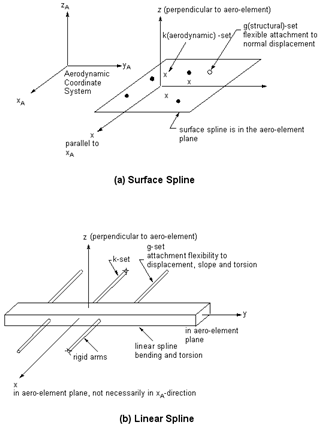
\includegraphics[width=0.6\linewidth]{figures/splines.png}
\fonte{\cite{patrannastran_aeroelastic_2019}}
\label{fig-splines}
\end{figure}

\subsection{Método de Solução Aeroelástica}

O MSC/NASTRAN fornece 6 métodos de solução aeroelástica para \emph{flutter}
o método americano \emph{K-method}; o \emph{KE-method}; o inglês \emph{PK-method}; o \emph{PKNL-method}; o \emph{PKS-method}; e o \emph{PKNLS-method}. Um resumo das características de cada método
está disposto na Tabela \ref{nastran-sol-table}.


\begin{table}[H]
\centering
\caption{Resumo de características dos métodos de solução aeroelástica.}
\begin{tabular}{|l|l|l|l|}
\hline
Método & Descrição & Entradas & Saídas \\ \hline
K      & Método iterativo americano clássico. & Conjuntos de $M$, $k$ e $\rho$   & $V$, $g$ e $f$.             \\ \hline
KE     & \begin{tabular}[c]{@{}l@{}}Variação do \emph{K-method}, desconsiderando\\ todos os amortecimentos viscosos, e com\\ uma solução somente em auto-valores.\end{tabular} & Conjuntos de $M$, $k$ e $\rho$   & $V$, $g$ e $f$.             \\ \hline
PK     & Método iterativo inglês clássico. & Combinações de $V$, $M$ e $\rho$ & $V$, $\gamma$ e $f$.         \\ \hline
PKNL   & \begin{tabular}[c]{@{}l@{}}Variação do \emph{PK-method} utilizando somente\\ conjuntos ordenados de entrada.\end{tabular}                                              & Conjuntos de $V$, $M$ e $\rho$   &$V$, $\gamma$ e $f$.         \\ \hline
PKS    & \begin{tabular}[c]{@{}l@{}}Variação do \emph{PK-method} não iterativa,\\ realizando uma "varredura" em uma faixa\\ de frequências reduzidas.\end{tabular}               & Combinações de $V$, $M$ e $\rho$ &$V$, $\gamma$ e $f$.         \\ \hline
PKNLS  & \begin{tabular}[c]{@{}l@{}}Variação do \emph{PKNL-method} não iterativa,\\ utilizando a mesma técnica do \emph{PKS-method}.\end{tabular}                                       & Conjuntos de $V$, $M$ e $\rho$   & $V$, $\gamma$ e $f$.         \\ \hline
\end{tabular}
\fonte{\cite{patrannastran_aeroelastic_2019}}
\label{nastran-sol-table}
\end{table}

Algumas comparações entre os métodos podem ser feitas.
Nos métodos tipo \emph{PK} há a inserção direta das velocidades,
o que é preferível, diferente dos métodos tipo \emph{K}, que
necessita um processo de ordenação dos resultados.
Nos métodos não iterativos, não há possibilidade de falha por
uma iteração indevida. Por fim, segundo 
\cite{rodden_mscnastran_1994}, o parâmetro de amortecimento 
$\gamma$ nos métodos tipo \emph{PK} é fisicamente mais significativo
que o parâmetro $g$ nos métodos tipo \emph{K}.
